% -- Encoding UTF-8 without BOM
% -- XeLaTeX => PDF (BIBER)

\documentclass[]{cv-style}          % Add 'print' as an option into the square bracket to remove colours from this template for printing. 
                                    % Add 'espanol' as an option into the square bracket to change the date format of the Last Updated Text

\sethyphenation[variant=british]{english}{} % Add words between the {} to avoid them to be cut 
\usepackage{graphicx}
\begin{document}

\header{Rafael de Moura }{Moreira}           % Your name
\lastupdated

%----------------------------------------------------------------------------------------
%	SIDEBAR SECTION  -- In the aside, each new line forces a line break
%----------------------------------------------------------------------------------------

\begin{aside}
\section{.}
\flushleft%
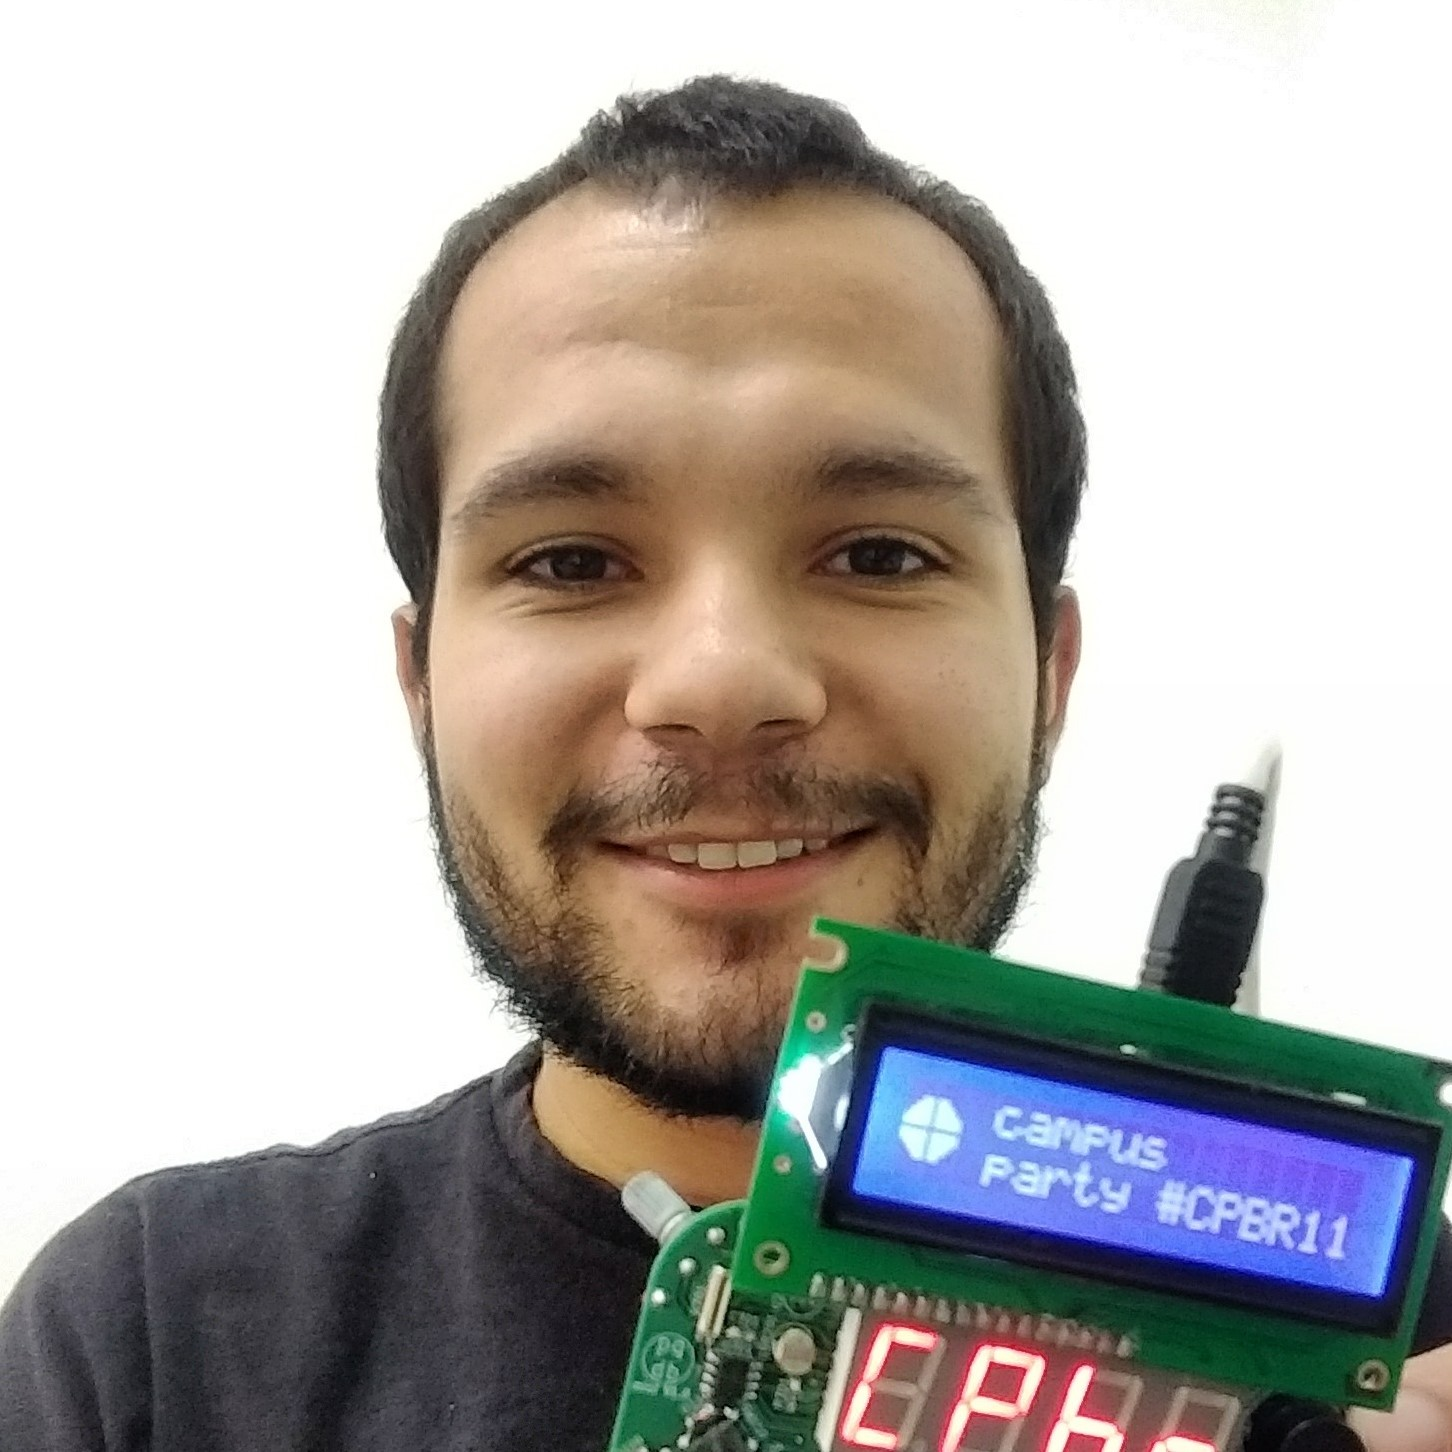
\includegraphics[width=4cm]{photo}
\section{Contact Information}
\href{https://wa.me/5511945545955}{+55 11 94554 5955}
~
\href{mailto:rafaelmmoreira@gmail.com}{rafaelmmoreira@gmail.com}
~
\url{https://www.linkedin.com/in/rafaelmmoreira/}
~
\url{https://github.com/rafaelmmoreira/}
%
\section{Languages}
Portuguese: native
English: fluent
Spanish: advanced
French: basic reading
%
\section{Professional interests}
Software development
Hardware prototyping
Data analysis
STEM education and popularization
%
\vspace{3.7cm}
The most recent version of this CV is available at:

\includegraphics[width=4cm]{qrcode}
Disponível em Português.
Disponible en Español.
%
\end{aside}

%----------------------------------------------------------------------------------------
%	SKILLS SECTION
%----------------------------------------------------------------------------------------

\section{Education}
\vspace{-0.3cm}
\begin{entrylist}
\entry
{}
{\textbf{Master of Science in Computer Science and Technology}}
{}
{\textit{ Federal University of Itajubá, 2019.}}
{}

\entry
{}
{\textbf{Bachelor of Science in Computer Engineering }}
{}
{\textit{ Federal University of Itajubá, 2015.}}
{}

\entry
{}
{\textbf{Graduate Course in Data Science}}
{}
{\textit{University Center of United Metropolitan Colleges (in progress).}}
{}

\entry
{}
{\textbf{Graduate Course in Software Development with Agile Methodologies}}
{}
{\textit{Anhembi Morumbi University (in progress).}}
{}

\end{entrylist}
{\vspace{-0.8cm}}
%	WORK EXPERIENCE SECTION
%----------------------------------------------------------------------------------------

\section{Experience}
\vspace{-0.3cm}
\begin{entrylist}
%------------------------------------------------


%----------------------------------------------------------------------------------------
\entry
{}
{Programmer | Setis Automação e Sistemas (PayGo/C6 Bank) | oct/18 - present}
{\vspace{-0.01cm}}
{Embedded software development and maintenance for several different models of POS terminals (credit card machines) for a major acquirer in Brazil using C language and Scrum. Development of automated package generation tools in Python.}
{}
 %----------------------------------------------------------------------------------------

\entry
  {}
  {Programming teacher | Let's Code Academy | jan/19 - present}
  {\vspace{-0.01cm}}
{Python Pro teacher: introduction to algorithms data structures, object oriented programming, GUI, APIs and web scraping. Wrote a full textbook for the course, plus a chapter on data visualization for the Data Science course textbook.}
 {} %----------------------------------------------------------------------------------------

\entry
  {}
  {Temporary Lecturer | Federal University of Itajubá | feb/17 - oct/18}
{\vspace{-0.01cm}}
{ Lecturer on Introduction to Programming on three undergraduate courses: Computer Engineering, Electronics Engineering and Control and Automation Engineering. Lessons in C and Python. Mentoring of two extracurricular projects: Dev-U (a videogame programming group for undergraduate students) and ProgramAção (undergraduate students teaching programming to high school students). }
 %----------------------------------------------------------------------------------------
\end{entrylist}
{\vspace{-0.4cm}}

\section{Public lectures and workshops}
\vspace{-0.3cm}
\begin{entrylist}

\entry
{}
{Most relevant lectures and workshops (all in Portuguese):}
{}
{\vspace{-0.5cm}}

%------------------------------------------------
\entry
{}
{\href{https://www.slideshare.net/rafaelmmoreira/como-fazer-seu-prprio-gameboy-cpbr11}{How to Make Your Own Gameboy}}
{\href{https://campuse.ro/events/campus-party-brasil-2018/workshop/como-fazer-seu-proprio-gameboy-cpbr11/}{Campus Party Brasil, 2018}}
{\vspace{-0.5cm}}
%------------------------------------------------
\entry
{}
{\href{https://www.slideshare.net/rafaelmmoreira/desenvolvimento-de-sistemas-embarcados-do-hardware-ao-software}{Embedded Systems Development}}
{\href{https://sp13.securitybsides.com.br/detalhe-dos-treinamentos-e-apresentacoes/}{BSides São Paulo, 2016}}
{\vspace{-0.5cm}}
%------------------------------------------------
\entry
{}
{\href{https://www.slideshare.net/rafaelmmoreira/escalonador-earliest-deadline-first-tdc2014sp}{Earliest Deadline First Scheduler}}
{\href{https://thedevconf.com/tdc/2014/saopaulo/trilha-embedded}{The Developer's Conference São Paulo, 2014}}
{\vspace{-0.5cm}}
%------------------------------------------------
\entry
{}
{\href{https://www.slideshare.net/rafaelmmoreira/programao-segura}{Secure Coding}}
{\href{https://garoa.net.br/wiki/O_Outro_Lado_BSidesSP_ed_naovaitercopa/Lightning_Talks}{BSides São Paulo, 2014}}
{\vspace{-0.5cm}}
%------------------------------------------------

%------------------------------------------------
\end{entrylist}
{\vspace{-0.2cm}}
%-------------------------------  ---------------------------------------------------------
%	END HOBBIES SECTION SECTION

\section{Published Articles}
\vspace{-0.3cm}
\begin{entrylist}
%------------------------------------------------
\entry
{}
{}
{\vspace{-0.4cm}}
{\href{https://doi.org/10.1109/ICM48031.2019.9021277}{Moreira, Rafael, et al. "Online Heartbeat Classification Using Low Cost Algorithms." \textit{2019 31st International Conference on Microelectronics (ICM)}. IEEE, 2019.}}
{}
%------------------------------------------------
\entry
{}
{}
{\vspace{-0.5cm}}
{\href{http://www.swge.inf.br/CBA2014/anais/PDF/1569927865.pdf}{Moreira, Rafael M., et al. "Plataforma Didatica de Baixo Custo para Experiências em Laboratorios de Controle (Low Cost Learning Tools for Control Engineering Experiments)". \textit{XX Brazilian Conference on Automation. SBA, 2014.}}}
{}
\end{entrylist}
{\vspace{-0.4cm}}

%%%%%%%%%
\section{Programming languages and tools}
\vspace{-0.3cm}
\begin{entrylist}
\entry
{}
{Most used languages}
{C, Python}
{\vspace{-0.5cm}}
\entry
{}
{Data modeling and analysis tools}
{Anaconda (Python), MATLAB, Octave}
{\vspace{-0.5cm}}
\entry
{}
{Microcontrollers and development boards}
{Arduino, Raspberry Pi, HCS12, PIC18F}
{\vspace{-0.5cm}}
\entry
{}
{Agile frameworks}
{Scrum, XP}
{\vspace{-0.5cm}}
\entry
{}
{Software versioning}
{GitHub}
{\vspace{-0.5cm}}
\entry
{}
{Different degrees of experience in other languages. Quick to learn how to use new tools and languages. }
{}
{\vspace{-4.0cm}}
\end{entrylist}


\end{document}
